% ============================================================
%  CHAPITRE 3 — SPRINT 1 : AUTHENTIFICATION ET GESTION DES PROFILS
% ============================================================
\chapter{Sprint 1 : Authentification et Gestion des Profils}

\chapintro{Ce premier sprint pose les fondations de la plateforme en implémentant
le système d'authentification sécurisé par JWT et la gestion des profils. Il
constitue le prérequis de toutes les fonctionnalités ultérieures.}

\section{Introduction}

L'authentification est le socle de toute plateforme multi-utilisateurs. Elle garantit
que chaque acteur accède uniquement aux ressources qui lui sont attribuées selon son
rôle. Ce sprint implémente un système JWT stateless, adapté au déploiement multi-tenant
et à l'architecture découplée front-end/back-end.

\section{Identification du Backlog Sprint 1}

\begin{table}[H]
\centering
\caption{Backlog Sprint 1 --- Authentification}
\label{tab:backlog-s1}
\begin{tabularx}{\textwidth}{|l|X|l|c|}
\hline
\rowcolor{gray!20}
\textbf{ID} & \textbf{User Story} & \textbf{Priorité} & \textbf{SP} \\
\hline
US01 & En tant qu'utilisateur, je veux m'inscrire avec email et mot de passe & \prio{H} & 3 \\[3pt]\hline
US02 & En tant qu'utilisateur, je veux me connecter et recevoir un JWT & \prio{H} & 3 \\[3pt]\hline
US03 & En tant qu'utilisateur, je veux que mon token se rafraîchisse automatiquement & \prio{H} & 2 \\[3pt]\hline
US04 & En tant qu'utilisateur, je veux modifier mon mot de passe & \prio{M} & 2 \\[3pt]\hline
\multicolumn{3}{|r|}{\textbf{Total Sprint 1}} & \textbf{10 SP} \\
\hline
\end{tabularx}
\end{table}

\noindent\textbf{Tâches techniques~:}
\begin{enumerate}[noitemsep]
  \item Modèles de domaine \texttt{User} et \texttt{Tenant}.
  \item Commandes CQRS~: \texttt{RegisterCommand}, \texttt{LoginCommand},
    \texttt{RefreshTokenCommand}, \texttt{ChangePasswordCommand}.
  \item Middleware JWT et filtre global multi-tenant EF Core.
  \item Endpoints REST dans \texttt{AuthController}.
  \item Écrans Angular~: \texttt{LoginComponent}, \texttt{SignupComponent}.
  \item Intercepteur HTTP pour injection automatique du Bearer Token.
\end{enumerate}

\section{Conception}

\subsection{Diagramme de cas d'utilisation --- Sprint 1}

\begin{figure}[H]
\centering
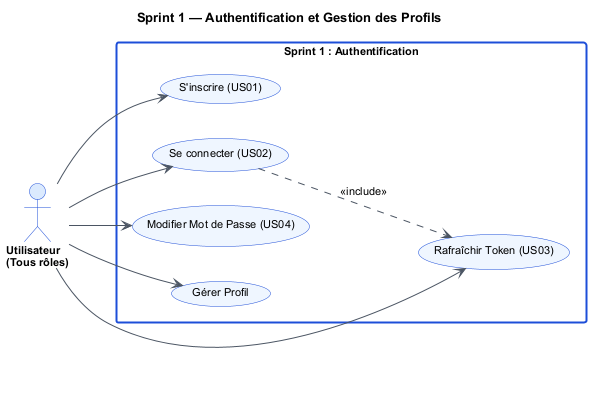
\includegraphics[width=0.82\textwidth]{diagrams/uc_s1.png}
\caption{Diagramme de cas d'utilisation --- Sprint 1}
\label{fig:uc-s1}
\end{figure}

\subsection{Diagramme de classes --- Sprint 1}

\begin{figure}[H]
\centering
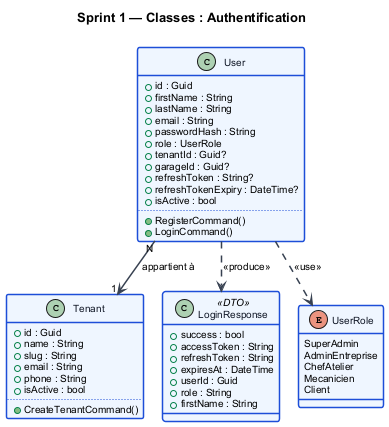
\includegraphics[width=\textwidth,height=0.62\textheight,keepaspectratio]{diagrams/class_s1.png}
\caption{Diagramme de classes --- Sprint 1 (Authentification)}
\label{fig:class-s1}
\end{figure}

\subsection{Diagramme de séquence}

\subsubsection*{SC1 --- Connexion (US02) : fonctionnalité principale}

\noindent L'utilisateur saisit ses identifiants. Le système valide, génère un JWT
et un refresh token, les stocke en base, et les retourne au client.

\begin{sidewaysfigure}[p]
\centering
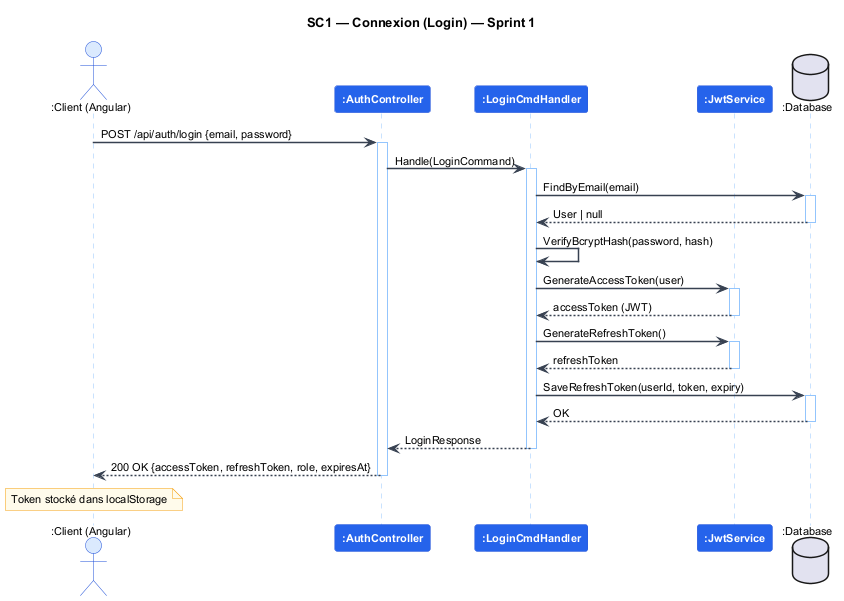
\includegraphics[width=0.92\textheight,keepaspectratio]{diagrams/seq_s1_login.png}
\caption{Diagramme de séquence SC1 --- Connexion (Login)}
\label{fig:seq-s1-login}
\end{sidewaysfigure}

\section{Conclusion}

Le Sprint 1 a établi l'infrastructure d'authentification complète de MecaRage.
Le système JWT est opérationnel avec gestion du refresh token, isolation multi-tenant
par filtre global EF Core (\texttt{HasQueryFilter}), et hachage BCrypt des mots de
passe. Les interfaces Angular de connexion et d'inscription sont déployées avec
support du mode sombre (dark mode Tailwind CSS).

Le Sprint 1 a établi l'infrastructure d'authentification complète de MecaRage.
Le système JWT est opérationnel avec gestion du refresh token, isolation multi-tenant
par filtre global EF Core (\texttt{HasQueryFilter}), et hachage BCrypt des mots de
passe. Les interfaces Angular de connexion et d'inscription sont déployées avec
support du mode sombre (dark mode Tailwind CSS).

